On peut définir la matrice $A$ avec la commande suivante

\begin{verbatim}
n=10;
A=2*diag(ones(1,n))-diag(ones(1,n-1),1)-diag(ones(1,n-1),-1);
A
\end{verbatim}

Après, on calcule son déterminant par

\begin{verbatim}
det(A)

ans = 11
\end{verbatim}

et les normes $\norm{A}_{1}$, $\norm{A}_{2}$, $\norm{A}_{\infty}$ par

\begin{verbatim}
nrm1=norm(A,1)
nrm2=norm(A,2)
nrminf=norm(A,inf)
\end{verbatim}

et on obtient

\begin{verbatim}
nrml = 4
nrm2 = 3.9190
nrminf = 4
\end{verbatim}


Pour évaluer le rayon spectral de $A$, il faut calculer ses valeurs propres et en prendre le maximum, en valeur absolue :
 
\begin{verbatim}
rho=max(abs(eig(A)))

rho = 3.9190
\end{verbatim}
 
On peut directement vérifier que, $A$ étant symétrique et définie positive, on a $\rho \parent{A} = \norm{A}_{2}$.
Pour calculer et visualiser les vecteurs propres $\BoldV_{j}, j \in \bracket{1, \dots, 10}$, il faut utiliser les commandes

\begin{verbatim}
[V, D]=eig(A);
figure
plot(V)
\end{verbatim}


ou, si on veut visualiser chaque vecteur propre individuellement, la boucle suivante :
 
\begin{verbatim}
figure
for i=1:10
    plot(V(:,i))
    pause
end
\end{verbatim}

Avec la première option, on a le graphe de la Figure \ref{fig:comp}.

\begin{figure}[h!]
  \centering
  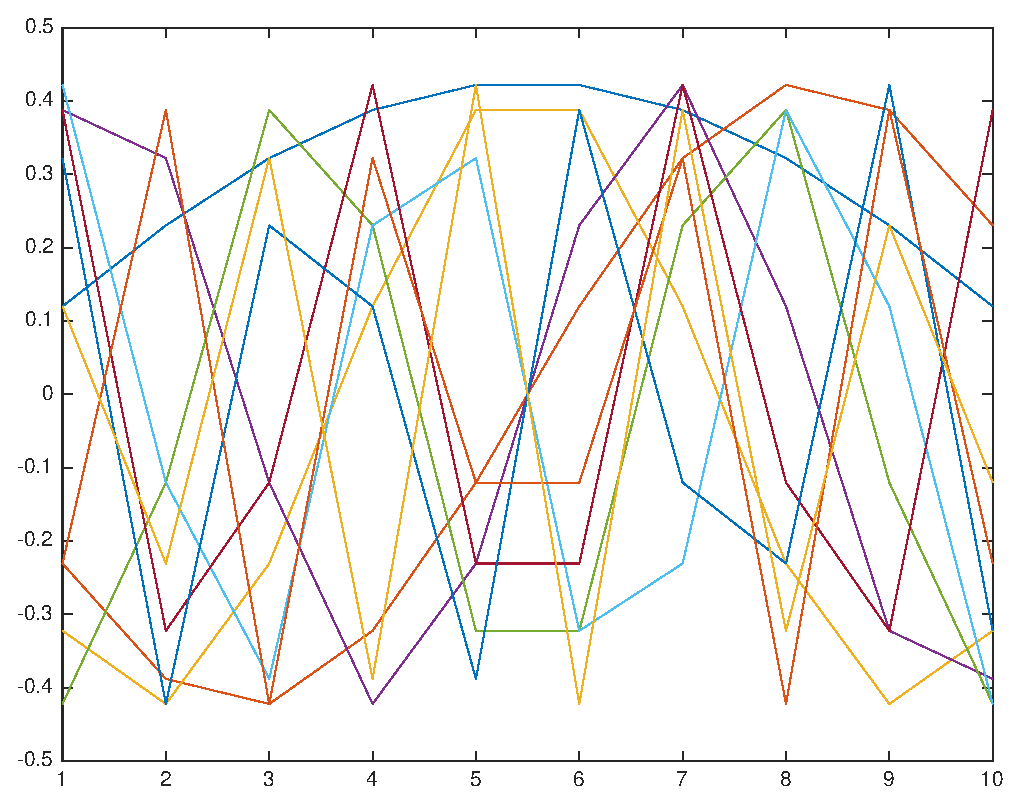
\includegraphics[scale = 0.5]{s1/matlab/comp.eps}
  \caption{Composantes des vecteurs propres de la matrice $A$.}
  \label{fig:comp}
\end{figure}


Pour vérifier que la matrice $V$ (dont les colonnes sont égales aux vecteurs propres de $A$) permet de diagonaliser la matrice $A$, c'est-à-dire $V^{-1} A V = D = \text{diag} \bracket{\lambda_{1}, \dots, \lambda_{n}}$, il faut utiliser les commandes suivantes :


\begin{verbatim}
[V,D]=eig(A)
inv(V)*A*V % ou mieux (V\A)*V
D
dif = norm(D-inv(V)*A*V); % ou mieux dif = norm(D-(V\A)*V);
\end{verbatim}

on obtient

\begin{verbatim}
dif = 3.5003e-15
\end{verbatim}

Enfin, pour visualiser la structure des matrices \texttt{A}, \texttt{V}, \texttt{D}, il faut taper

\begin{verbatim}
spy(A)
spy(D)
spy(V)
\end{verbatim}

On peut observer à la Figure \ref{fig:structure} que la matrice $A$ est tri-diagonale, la matrice $D$ est diagonale alors que la matrice $V$ des vecteurs propres est pleine : tous ses éléments sont différentes de zéro.

 





\begin{figure}[h!]
  \begin{subfigure}[b]{0.3\linewidth}
    \centering
    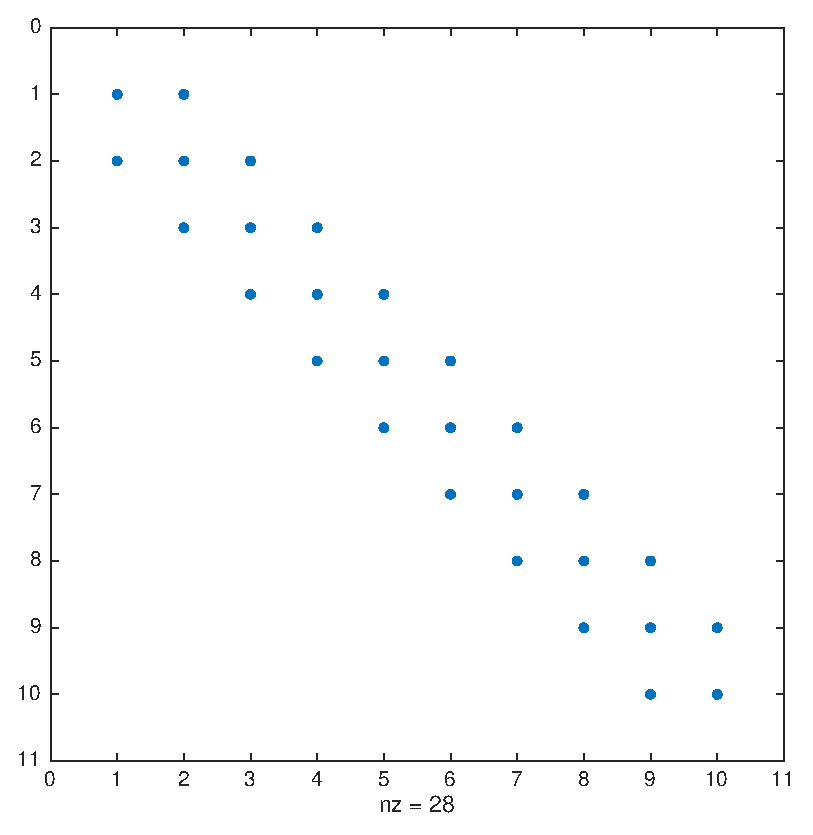
\includegraphics[scale=0.2]{s1/matlab/A} 
    %\caption{Interpolation of $f$ using NCS \\ with $7+2$ points} 
    %\label{fig:q11_n7} 
  \end{subfigure}
  \begin{subfigure}[b]{0.3\linewidth}
    \centering
    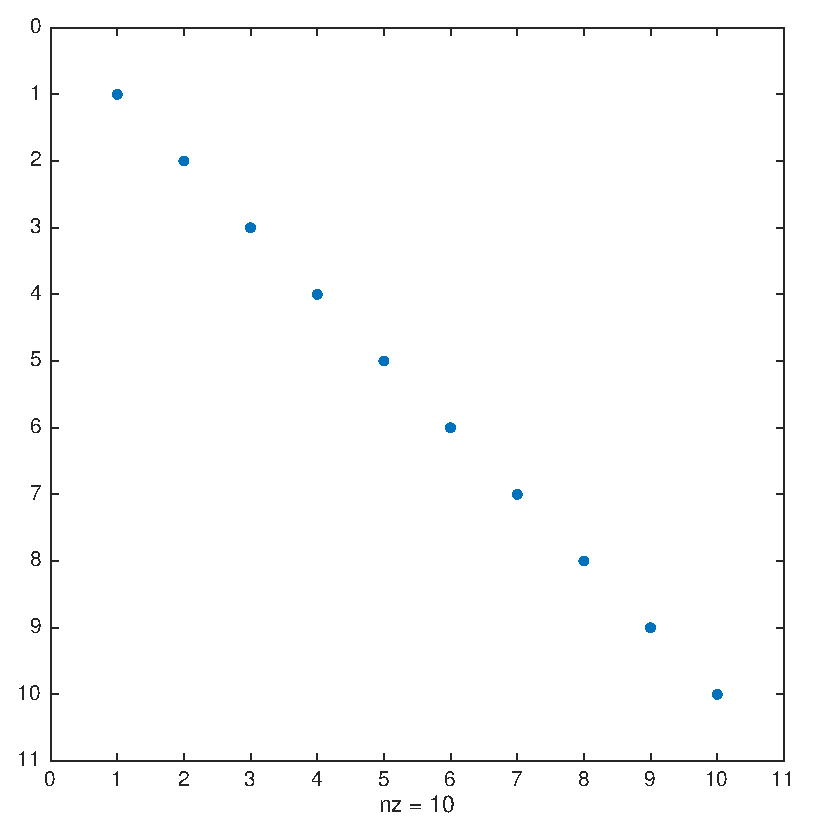
\includegraphics[scale=0.2]{s1/matlab/D} 
    %\caption{Interpolation of $f$ using NCS \\ with $8+2$ points} 
    %\label{fig:q11_n8} 
  \end{subfigure}
  \begin{subfigure}[b]{0.3\linewidth}
    \centering
    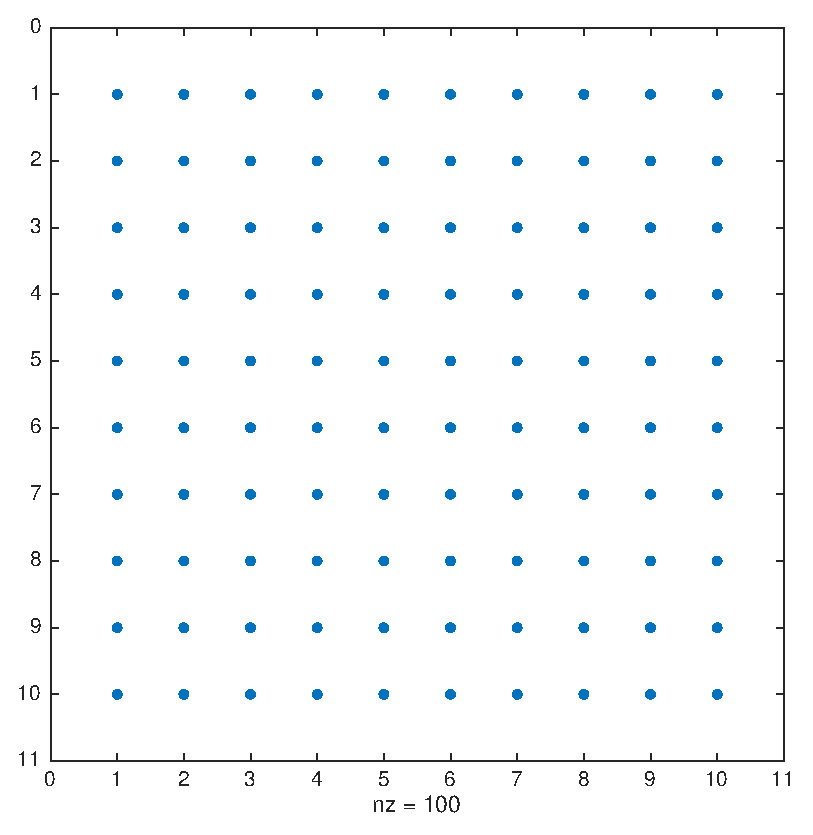
\includegraphics[scale=0.2]{s1/matlab/V} 
    %\caption{Interpolation of $f$ using NCS \\ with $8+2$ points} 
    %\label{fig:q11_n8} 
  \end{subfigure} 
  \caption{Structure des matrices $A$, $D$ et $V$ de gauche à droite.}
  \label{fig:structure}
\end{figure}


